% Draft preprint. Every number is a macro from numbers.tex / tables.tex, generated by make_numbers.py from the result
% files in ../results. Re-run `python paper/make_numbers.py` after any new result, then rebuild.
\documentclass[11pt]{article}
\usepackage[a4paper,margin=2.3cm]{geometry}
\usepackage[T1]{fontenc}
\usepackage{lmodern}
\usepackage{amsmath,amssymb}
\usepackage{booktabs}
\usepackage{graphicx}
\usepackage{caption}
\usepackage{xcolor}
\usepackage[hidelinks]{hyperref}
\usepackage{url}
\newcommand{\OrigDegAuroc}{0.946}
\newcommand{\OrigFA}{22.5\%}
\newcommand{\OrigWorstFA}{63\%}
\newcommand{\OrigTPR}{87.9\%}
\newcommand{\OrigBacc}{82.7\%}
\newcommand{\OrigPooled}{0.920}
\newcommand{\OrigTprFive}{67.2\%}
\newcommand{\OrigTprTen}{77.6\%}
\newcommand{\OrigCleanFA}{2.9\%}
\newcommand{\OrigConFA}{22.5\%}
\newcommand{\OrigCvFA}{22.5\%}
\newcommand{\PlattDegAuroc}{0.942}
\newcommand{\PlattFA}{12.2\%}
\newcommand{\PlattWorstFA}{49\%}
\newcommand{\PlattTPR}{81.5\%}
\newcommand{\PlattBacc}{84.7\%}
\newcommand{\PlattPooled}{0.917}
\newcommand{\PlattTprFive}{67.1\%}
\newcommand{\PlattTprTen}{78.3\%}
\newcommand{\PlattCleanFA}{0.0\%}
\newcommand{\PlattConFA}{12.2\%}
\newcommand{\PlattCvFA}{15.3\%}
\newcommand{\SCDegAuroc}{0.945}
\newcommand{\SCFA}{8.7\%}
\newcommand{\SCWorstFA}{44\%}
\newcommand{\SCTPR}{78.1\%}
\newcommand{\SCBacc}{84.7\%}
\newcommand{\SCPooled}{0.951}
\newcommand{\SCTprFive}{71.0\%}
\newcommand{\SCTprTen}{80.5\%}
\newcommand{\SCCleanFA}{1.4\%}
\newcommand{\SCConFA}{6.9\%}
\newcommand{\SCCvFA}{7.8\%}
\newcommand{\StrictDegAuroc}{0.938}
\newcommand{\StrictFA}{2.3\%}
\newcommand{\StrictWorstFA}{14\%}
\newcommand{\StrictTPR}{61.4\%}
\newcommand{\StrictBacc}{79.6\%}
\newcommand{\StrictPooled}{0.951}
\newcommand{\StrictTprFive}{71.0\%}
\newcommand{\StrictTprTen}{80.0\%}
\newcommand{\StrictCleanFA}{0.0\%}
\newcommand{\StrictConFA}{2.4\%}
\newcommand{\StrictCvFA}{1.4\%}
\newcommand{\QsDegAuroc}{0.938}
\newcommand{\QsFA}{15.1\%}
\newcommand{\QsWorstFA}{69\%}
\newcommand{\QsTPR}{86.2\%}
\newcommand{\QsBacc}{85.5\%}
\newcommand{\QsPooled}{0.954}
\newcommand{\QsTprFive}{59.7\%}
\newcommand{\QsTprTen}{79.1\%}
\newcommand{\QsCleanFA}{2.9\%}
\newcommand{\QsConFA}{8.4\%}
\newcommand{\QsCvFA}{16.4\%}
\newcommand{\RefitDegAuroc}{0.880}
\newcommand{\RefitFA}{8.0\%}
\newcommand{\RefitWorstFA}{31\%}
\newcommand{\RefitTPR}{68.8\%}
\newcommand{\RefitBacc}{80.4\%}
\newcommand{\RefitPooled}{0.892}
\newcommand{\RefitTprFive}{62.7\%}
\newcommand{\RefitTprTen}{70.1\%}
\newcommand{\RefitCleanFA}{4.3\%}
\newcommand{\RefitConFA}{8.0\%}
\newcommand{\RefitCvFA}{17.3\%}
\newcommand{\OrigFAGBFive}{63\%}
\newcommand{\OrigAurocGBFive}{0.905}
\newcommand{\SCFAGBFive}{11\%}
\newcommand{\SCTPRGBFive}{73\%}
\newcommand{\OrigTPRGBFive}{98\%}
\newcommand{\OrigFAVCFive}{33\%}
\newcommand{\OrigAurocVCFive}{0.879}
\newcommand{\SCFAVCFive}{13\%}
\newcommand{\SCTPRVCFive}{72\%}
\newcommand{\OrigTPRVCFive}{88\%}
\newcommand{\OrigFAJPEGFive}{59\%}
\newcommand{\OrigAurocJPEGFive}{0.885}
\newcommand{\SCFAJPEGFive}{44\%}
\newcommand{\SCTPRJPEGFive}{90\%}
\newcommand{\OrigTPRJPEGFive}{95\%}
\newcommand{\OrigFAclean}{3\%}
\newcommand{\OrigAurocclean}{0.999}
\newcommand{\SCFAclean}{1\%}
\newcommand{\SCTPRclean}{98\%}
\newcommand{\OrigTPRclean}{98\%}
\newcommand{\ProbeReal}{$+1.44$}
\newcommand{\ProbeFake}{$-0.17$}
\newcommand{\ProbeAuroc}{0.992}
\newcommand{\FpAcc}{77.2\%}
\newcommand{\FpLogit}{57.0\%}
\newcommand{\FpN}{79}
\newcommand{\ClipRawFAFfppclean}{16\%}
\newcommand{\ClipCalFAFfppclean}{13\%}
\newcommand{\ClipRawBaccFfppclean}{90.5\%}
\newcommand{\ClipCalBaccFfppclean}{91.1\%}
\newcommand{\ClipRawAurocFfppclean}{0.986}
\newcommand{\ClipCalAurocFfppclean}{0.985}
\newcommand{\ClipRawFAFfppGBFive}{96\%}
\newcommand{\ClipCalFAFfppGBFive}{30\%}
\newcommand{\ClipRawBaccFfppGBFive}{51.3\%}
\newcommand{\ClipCalBaccFfppGBFive}{71.7\%}
\newcommand{\ClipRawAurocFfppGBFive}{0.788}
\newcommand{\ClipCalAurocFfppGBFive}{0.765}
\newcommand{\ClipRawFAFfppVCFive}{71\%}
\newcommand{\ClipCalFAFfppVCFive}{60\%}
\newcommand{\ClipRawBaccFfppVCFive}{59.3\%}
\newcommand{\ClipCalBaccFfppVCFive}{63.3\%}
\newcommand{\ClipRawAurocFfppVCFive}{0.798}
\newcommand{\ClipCalAurocFfppVCFive}{0.802}
\newcommand{\ClipRawFADfdcclean}{72\%}
\newcommand{\ClipCalFADfdcclean}{55\%}
\newcommand{\ClipRawBaccDfdcclean}{58.8\%}
\newcommand{\ClipCalBaccDfdcclean}{66.2\%}
\newcommand{\ClipRawAurocDfdcclean}{0.815}
\newcommand{\ClipCalAurocDfdcclean}{0.834}
\newcommand{\ClipRawFADfdcGBFive}{100\%}
\newcommand{\ClipCalFADfdcGBFive}{75\%}
\newcommand{\ClipRawBaccDfdcGBFive}{50.0\%}
\newcommand{\ClipCalBaccDfdcGBFive}{51.2\%}
\newcommand{\ClipRawAurocDfdcGBFive}{0.562}
\newcommand{\ClipCalAurocDfdcGBFive}{0.559}
\newcommand{\ClipRawFADfdcVCFive}{98\%}
\newcommand{\ClipCalFADfdcVCFive}{72\%}
\newcommand{\ClipRawBaccDfdcVCFive}{50.0\%}
\newcommand{\ClipCalBaccDfdcVCFive}{55.0\%}
\newcommand{\ClipRawAurocDfdcVCFive}{0.571}
\newcommand{\ClipCalAurocDfdcVCFive}{0.573}
\newcommand{\PeRawFAFfppclean}{9\%}
\newcommand{\PeCalFAFfppclean}{7\%}
\newcommand{\PeRawBaccFfppclean}{95.7\%}
\newcommand{\PeCalBaccFfppclean}{96.4\%}
\newcommand{\PeRawAurocFfppclean}{0.998}
\newcommand{\PeCalAurocFfppclean}{0.998}
\newcommand{\PeRawFAFfppGBFive}{86\%}
\newcommand{\PeCalFAFfppGBFive}{31\%}
\newcommand{\PeRawBaccFfppGBFive}{56.3\%}
\newcommand{\PeCalBaccFfppGBFive}{70.1\%}
\newcommand{\PeRawAurocFfppGBFive}{0.807}
\newcommand{\PeCalAurocFfppGBFive}{0.827}
\newcommand{\PeRawFAFfppVCFive}{51\%}
\newcommand{\PeCalFAFfppVCFive}{40\%}
\newcommand{\PeRawBaccFfppVCFive}{66.8\%}
\newcommand{\PeCalBaccFfppVCFive}{71.7\%}
\newcommand{\PeRawAurocFfppVCFive}{0.814}
\newcommand{\PeCalAurocFfppVCFive}{0.816}
\newcommand{\PeRawFADfdcclean}{22\%}
\newcommand{\PeCalFADfdcclean}{10\%}
\newcommand{\PeRawBaccDfdcclean}{72.5\%}
\newcommand{\PeCalBaccDfdcclean}{70.0\%}
\newcommand{\PeRawAurocDfdcclean}{0.814}
\newcommand{\PeCalAurocDfdcclean}{0.809}
\newcommand{\PeRawFADfdcGBFive}{90\%}
\newcommand{\PeCalFADfdcGBFive}{22\%}
\newcommand{\PeRawBaccDfdcGBFive}{51.2\%}
\newcommand{\PeCalBaccDfdcGBFive}{58.8\%}
\newcommand{\PeRawAurocDfdcGBFive}{0.611}
\newcommand{\PeCalAurocDfdcGBFive}{0.625}
\newcommand{\PeRawFADfdcVCFive}{72\%}
\newcommand{\PeCalFADfdcVCFive}{52\%}
\newcommand{\PeRawBaccDfdcVCFive}{56.2\%}
\newcommand{\PeCalBaccDfdcVCFive}{61.3\%}
\newcommand{\PeRawAurocDfdcVCFive}{0.632}
\newcommand{\PeCalAurocDfdcVCFive}{0.674}
\newcommand{\NVal}{353}
\newcommand{\NewBaseBacc}{62.2\%}
\newcommand{\NewFinBacc}{85.0\%}
\newcommand{\NewGain}{$+22.8$}
\newcommand{\NewCiLo}{$+17.4$}
\newcommand{\NewCiHi}{$+28.3$}
\newcommand{\FfppBase}{84.6\%}
\newcommand{\FfppFin}{79.0\%}
\newcommand{\FfppChange}{$-5.6$}
\newcommand{\DfdcBase}{58.8\%}
\newcommand{\DfdcFin}{60.4\%}
\newcommand{\DfdcChange}{$+1.7$}
\newcommand{\FfppCleanFAFin}{18.6\%}
\newcommand{\FfppCleanFABase}{1.4\%}
\newcommand{\AllAcc}{85.1\%}
\newcommand{\AllAccBase}{63.1\%}
\newcommand{\AllN}{705}
\newcommand{\BandAAcc}{58.1\%}
\newcommand{\BandAShare}{12.2\%}
\newcommand{\BandBAcc}{76.4\%}
\newcommand{\BandBShare}{17.4\%}
\newcommand{\BandCAcc}{91.9\%}
\newcommand{\BandCShare}{70.4\%}
\newcommand{\PeftValBase}{0.719}
\newcommand{\PeftValBest}{0.919}

\newcommand{\TabRoundOne}{\begin{tabular}{lccccccc}
\toprule
Method & AUROC & FA@0.5 & worst FA & TPR@0.5 & bal.\ acc. & TPR@5\%FA & pooled AUROC \\
\midrule
Released DFD-FCG & 0.946 & 22.5\% & 63\% & 87.9\% & 82.7\% & 67.2\% & 0.920 \\
Platt recalibration & 0.942 & 12.2\% & 49\% & 81.5\% & 84.7\% & 67.1\% & 0.917 \\
Quality-regression shift & 0.938 & 15.1\% & 69\% & 86.2\% & 85.5\% & 59.7\% & 0.954 \\
Quality-augmented head re-fit & 0.880 & 8.0\% & 31\% & 68.8\% & 80.4\% & 62.7\% & 0.892 \\
Self-calibration (ours) & 0.945 & 8.7\% & 44\% & 78.1\% & 84.7\% & 71.0\% & 0.951 \\
Self-calibration + blur probe & 0.938 & 2.3\% & 14\% & 61.4\% & 79.6\% & 71.0\% & 0.951 \\
\bottomrule
\end{tabular}
}
\newcommand{\TabTransfer}{\begin{tabular}{lcccc}
\toprule
 & \multicolumn{2}{c}{GenD-CLIP} & \multicolumn{2}{c}{GenD-PE} \\
\cmidrule(lr){2-3}\cmidrule(lr){4-5}
Test videos & false alarms & AUROC & false alarms & AUROC \\
\midrule
FF++, as uploaded & 16\% $\rightarrow$ \textbf{13\%} & 0.986 $\rightarrow$ 0.985 & 9\% $\rightarrow$ \textbf{7\%} & 0.998 $\rightarrow$ 0.998 \\
DFDC, as uploaded & 72\% $\rightarrow$ \textbf{55\%} & 0.815 $\rightarrow$ 0.834 & 22\% $\rightarrow$ \textbf{10\%} & 0.814 $\rightarrow$ 0.809 \\
FF++, strong blur & 96\% $\rightarrow$ \textbf{30\%} & 0.788 $\rightarrow$ 0.765 & 86\% $\rightarrow$ \textbf{31\%} & 0.807 $\rightarrow$ 0.827 \\
DFDC, strong blur & 100\% $\rightarrow$ \textbf{75\%} & 0.562 $\rightarrow$ 0.559 & 90\% $\rightarrow$ \textbf{22\%} & 0.611 $\rightarrow$ 0.625 \\
FF++, heavy H.264 & 71\% $\rightarrow$ \textbf{60\%} & 0.798 $\rightarrow$ 0.802 & 51\% $\rightarrow$ \textbf{40\%} & 0.814 $\rightarrow$ 0.816 \\
DFDC, heavy H.264 & 98\% $\rightarrow$ \textbf{72\%} & 0.571 $\rightarrow$ 0.573 & 72\% $\rightarrow$ \textbf{52\%} & 0.632 $\rightarrow$ 0.674 \\
\bottomrule
\end{tabular}
}
\newcommand{\TabFusion}{\begin{tabular}{lrcccc}
\toprule
Held-out test set & $n$ & DFD-FCG + SC & GenD-PE & GenD-PE ft & Fused (live) \\
\midrule
Celeb-DF v2 (2020) & 120 & 78.3\% & 75.8\% & 90.0\% & \textbf{92.5\%} \\
Social-media deepfakes (2026) & 87 & 55.0\% & 63.8\% & \textbf{92.0\%} & 89.2\% \\
MAVOS-DD, seen methods (2025) & 78 & 54.7\% & 52.8\% & \textbf{87.4\%} & 83.4\% \\
MAVOS-DD, unseen methods (2025) & 56 & 60.7\% & 58.9\% & \textbf{76.8\%} & 75.0\% \\
SynthForensics$^\dagger$ (2026) & 59 & 35.6\% & 62.7\% & 57.6\% & \textbf{76.3\%} \\
AI talking heads$^\dagger$ (2026) & 80 & 15.0\% & 46.2\% & \textbf{100.0\%} & \textbf{100.0\%} \\
FF++ test$^\ast$ & 130 & \textbf{84.6\%} & 72.9\% & 78.9\% & 79.0\% \\
FaceShifter$^\ast$ & 85 & \textbf{70.5\%} & 66.8\% & 58.3\% & 63.5\% \\
DFDC part 0$^\ast$ & 80 & 58.8\% & 60.0\% & 57.5\% & \textbf{60.4\%} \\
\bottomrule
\end{tabular}
}

\graphicspath{{../results/figures/}}
\captionsetup{font=small,labelfont=bf}

\title{Fake, or Just Low Quality? Decision Collapse of Deepfake Detectors under Video Degradation, and a Training-Free Self-Calibration}
\author{Roshan Raj\\ \small Department of Computer Science and Engineering, \textcolor{red}{[Institution]}\\ \small \texttt{[email]}}
\date{Draft, November 2026}

\begin{document}
\maketitle

\begin{abstract}
Video deepfake detectors are usually reported robust to blur and compression because their AUROC stays high on
degraded video. We show that this hides a failure at the decision a user actually sees. Under the authors' own
perturbation protocol, the released DFD-FCG detector (CVPR 2025) keeps a mean AUROC of \OrigDegAuroc{} over 13
degraded conditions of the FaceForensics++ test split, yet calls \OrigFA{} of authentic videos fake at its threshold,
and \OrigFAGBFive{} under strong blur. We trace the cause inside the model: blurring the aligned face by 2\,px moves the
fusion logit by \ProbeReal{} on real videos and \ProbeFake{} on fakes, so fine natural detail acts as evidence of
authenticity, and every degradation removes it. We propose \emph{self-calibration}, a ridge read-out of the
detector's own features that predicts the class-agnostic fake evidence a degradation adds and subtracts it, with no
retraining. On degradation types withheld from fitting it lowers false alarms from \OrigFA{} to \SCFA{} and raises
the AUROC of all conditions ranked together from \OrigPooled{} to \SCPooled{}. The collapse is not specific to one
model: GenD (WACV 2026), a frame-level detector with a different backbone, calls \PeRawFAFfppGBFive{} (Perception
Encoder) and \ClipRawFAFfppGBFive{} (CLIP) of real FF++ videos fake under strong blur, and the same read-out recipe,
unchanged, reduces this to \PeCalFAFfppGBFive{} and \ClipCalFAFfppGBFive{}. Finally, we combine self-calibrated DFD-FCG
with a GenD model fine-tuned on 2025--2026 data in a public checker that always answers REAL or FAKE. On \AllN{}
held-out videos (nine test sets from seven public datasets) it is correct on \AllAcc{} of them, against \AllAccBase{} for the self-calibrated
DFD-FCG alone, at the cost of more false alarms on FaceForensics++, which we report.
\end{abstract}

\section{Introduction}
Most detectors are evaluated by the area under the ROC curve (AUROC), which measures whether fakes score higher than
real videos, irrespective of any threshold. A deployed detector, however, makes a decision at a fixed threshold, and
that decision is what a journalist or a viewer acts on. Robustness tables report AUROC per perturbation
\cite{han2025dfdfcg}; if a degradation shifts the scores of \emph{all} videos towards ``fake'', the ranking, and
therefore AUROC, can survive while the decisions do not.

We study this gap on DFD-FCG \cite{han2025dfdfcg}, a recent video detector built on a frozen CLIP ViT-L/14
\cite{radford2021clip}, and then on GenD \cite{yermakov2026gend}, a frame-level detector that tunes only the
LayerNorm parameters of CLIP or Perception Encoder \cite{bolya2025pe} backbones. Our contributions are:
\begin{enumerate}
  \item \textbf{A measured failure.} With the authors' perturbation code, degraded AUROC stays at \OrigDegAuroc{} while
        \OrigFA{} of real test videos are called fake at the released threshold (worst condition \OrigWorstFA{}).
  \item \textbf{Its mechanism.} An exact additive decomposition of DFD-FCG's three heads and a 2-px blur probe show that
        the model reads fine detail as evidence of authenticity (Sec.~\ref{sec:cause}).
  \item \textbf{A training-free fix that transfers.} Self-calibration lowers false alarms on unseen degradation types
        from \OrigFA{} to \SCFA{} for DFD-FCG and, applied unchanged, from \PeRawFAFfppGBFive{} to \PeCalFAFfppGBFive{} under
        strong blur for GenD-PE (Sec.~\ref{sec:selfcal}, \ref{sec:transfer}).
  \item \textbf{A public checker} combining both detector families, with the selection rules fixed before testing and
        the trade-offs reported, including the rule that it did not meet (Sec.~\ref{sec:fusion}).
\end{enumerate}

\section{Related work}
\textbf{Video deepfake detection with foundation models.} DFD-FCG \cite{han2025dfdfcg} adds a side network to a frozen
CLIP encoder, with four facial-component queries (eyes, nose, lips, skin) guided by a face-feature loss and a temporal
module, and three linear heads (spatial, temporal, fusion). GenD \cite{yermakov2026gend} shows that tuning only the
LayerNorm parameters, with an L2-normalised class token and alignment and uniformity losses \cite{wang2020alignment},
generalises across 14 benchmarks. Both are trained on FaceForensics++ \cite{rossler2019ffpp} and evaluated on
Celeb-DF \cite{li2020celebdf}, DFDC \cite{dolhansky2020dfdc} and others.

\textbf{Robustness and calibration.} Corruption benchmarks \cite{hendrycks2019benchmarking} report accuracy under
perturbations; deepfake papers usually report AUROC. Post-hoc calibration such as Platt scaling
\cite{platt1999probabilistic} or temperature scaling \cite{guo2017calibration} applies one global transform to all
inputs and cannot correct a shift whose size depends on how degraded each input is. Our read-out is input-dependent:
it estimates the shift of each video from that video's own features.

\section{Setting}
\label{sec:setting}
\textbf{Data.} The FaceForensics++ (c23) test split provides 70 real videos and 60 fakes (15 each of Deepfakes,
Face2Face, FaceSwap and NeuralTextures). We add 15 FaceShifter \cite{li2019faceshifter} fakes, a manipulation DFD-FCG
never saw, and 80 DFDC videos \cite{dolhansky2020dfdc} (training part 0, 40 real and 40 fake). The read-out is fitted on
49 disjoint FF++ \emph{training}-split videos.

\textbf{Degradations.} We use the authors' robustness code: colour saturation, colour contrast, block-wise occlusion,
Gaussian noise, Gaussian blur (GB), down/up-sampling and H.264 compression (VC). The three that cause false alarms
(blur, resampling, H.264) are tested at severities 1, 3 and 5, the others at 3; a re-encode-only control (RE) isolates
the codec round trip. The read-out is fitted at severities 2 and 4 only, and in the strictest protocol (``type
unseen'') the tested degradation type is also withheld from fitting.

\textbf{Metrics.} Besides AUROC we report, at the released threshold 0.5, the false-alarm rate (real videos called
fake, FA), the share of fakes caught (TPR) and balanced accuracy; the TPR at a matched 5\% FA budget; and the
\emph{pooled} AUROC, which ranks all conditions together, as a deployed detector must.

\section{AUROC hides a decision collapse}
\label{sec:collapse}
Figure~\ref{fig:collapse} and the first row of Table~\ref{tab:round1} show the gap. Mean AUROC over the 13 degraded
conditions is \OrigDegAuroc{}, yet \OrigFA{} of real videos are called fake on average. Under strong blur (GB$_5$)
AUROC is still \OrigAurocGBFive{} while \OrigFAGBFive{} of real videos are flagged; H.264 at severity 5 flags \OrigFAVCFive{}.
Gaussian noise does the opposite and hides fakes. A robustness table in AUROC alone reports none of this.

\begin{figure}[t]
  \centering
  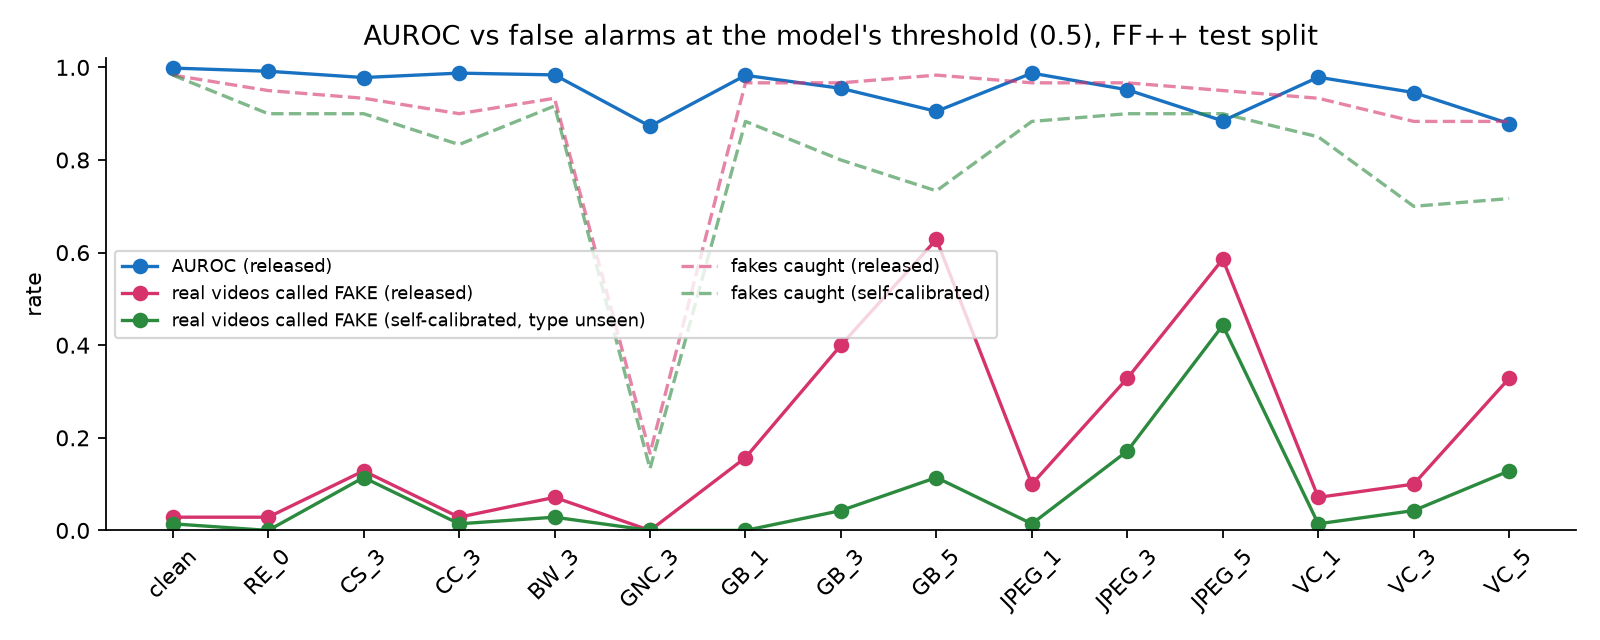
\includegraphics[width=\linewidth]{f1_collapse.png}
  \caption{FF++ test split, released DFD-FCG. AUROC (blue) stays high under degradation while the share of real
  videos called fake at the threshold (red) rises up to \OrigFAGBFive{}. Green: self-calibrated, with the tested
  degradation type withheld from fitting.}
  \label{fig:collapse}
\end{figure}

\section{Why: fine detail is read as evidence of authenticity}
\label{sec:cause}
\textbf{Exact attribution.} Each DFD-FCG head is linear after a LayerNorm, and the features it reads are sums over
layers, facial-component queries and patches. Because LayerNorm is affine once its statistics are fixed, every head
logit splits exactly into per-layer, per-component and per-patch terms plus a constant. Over all 5{,}976 analysed clips
the 240 layer$\times$component terms reproduce each head logit to $3\cdot10^{-7}$ (fp16 inference). From the
attribution of clean fakes alone, a linear classifier names the manipulation method of \FpN{} videos with \FpAcc{}
accuracy (identity-grouped 5-fold; \FpLogit{} from the three head logits, 25\% chance).

\textbf{Blur probe.} Blurring the aligned face by 2\,px changes the fusion logit by \ProbeReal{} on clean real videos
and by \ProbeFake{} on fakes (Fig.~\ref{fig:probe}); the response alone separates real from fake with AUROC
\ProbeAuroc{}. Real faces carry fine natural texture that the model counts as evidence of authenticity; current fakes
carry less of it. Every degradation removes that texture, so authentic videos drift towards ``fake''. On already
degraded input the probe gap shrinks, which is why the probe itself is a weak fix (Sec.~\ref{sec:negative}).

\begin{figure}[t]
  \centering
  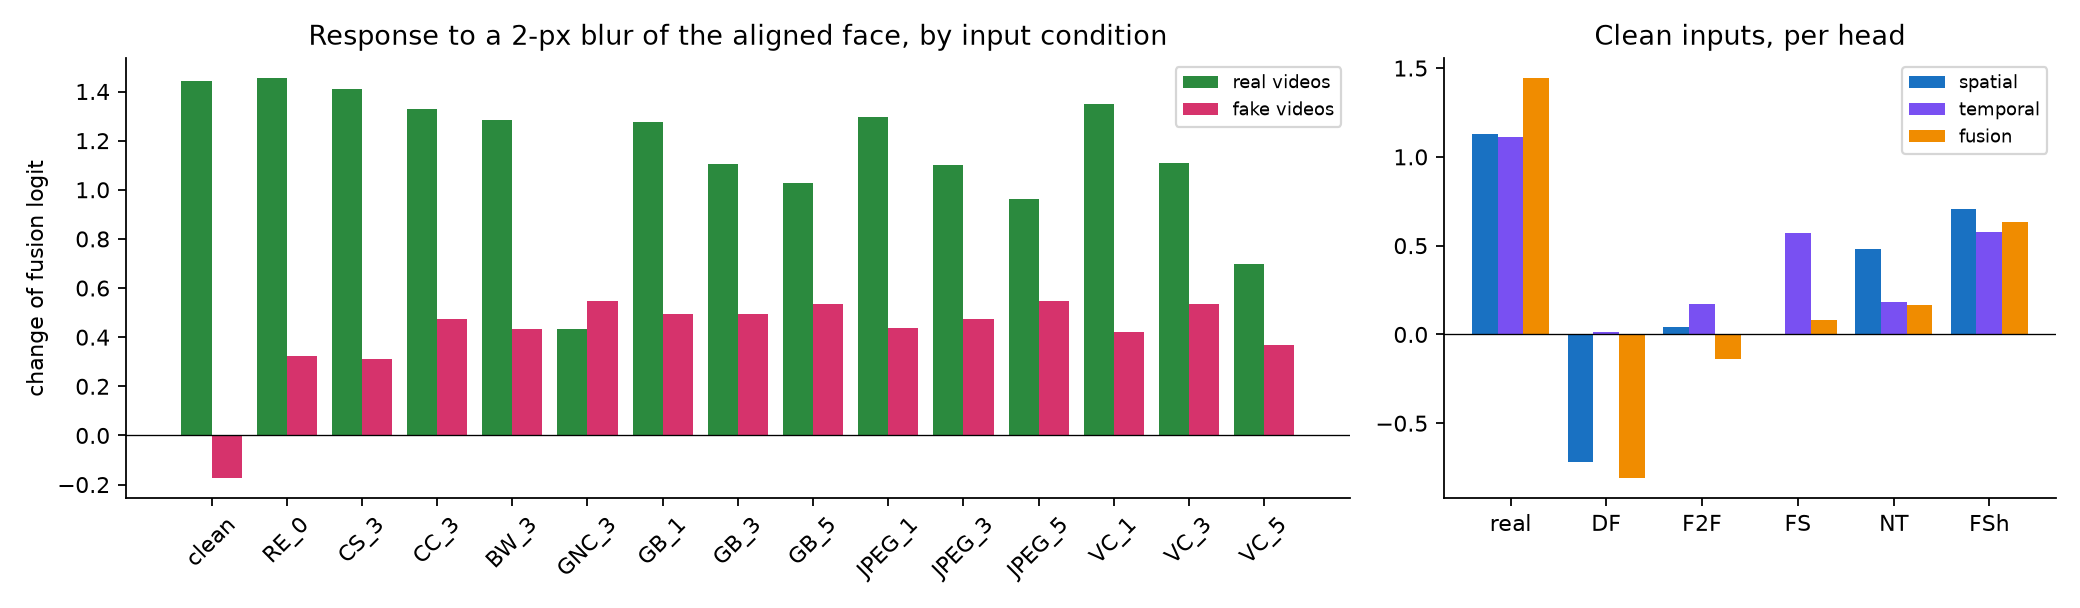
\includegraphics[width=\linewidth]{f4_fragility.png}
  \caption{Change of the fusion logit when the aligned face is blurred by 2\,px. Left: per input condition. Right:
  clean inputs, per head and manipulation method.}
  \label{fig:probe}
\end{figure}

\section{Self-calibration}
\label{sec:selfcal}
Let $\mathbf{y}=[\mathbf{y}_s,\mathbf{y}_t]$ be the 1024-d spatial and 256-d temporal features DFD-FCG's heads read, and
$d_h$ the logit (fake minus real) of head $h\in\{s,t,a\}$. A ridge read-out predicts the spurious evidence
\begin{equation}
  \mathbf{g} = W\,\mathrm{std}(\mathbf{y}) + \mathbf{b},\qquad d'_h = d_h - g_h,\qquad
  P = \tfrac13\textstyle\sum_h \sigma(d'_h),
\end{equation}
and the decision stays $P\ge0.5$. The training target is \emph{class-agnostic}: for a fit clip under condition $c$ it
is the mean paired shift $\mathbb{E}[d(c)-d(\text{clean})]$ that $c$ causes on the \emph{real} fit videos ($0$ for
clean), assigned to real and fake clips alike. The read-out therefore learns ``which degradation, how strong'', never
``real or fake''. Ridge strength $\alpha=1000$ on standardised features. The released checkpoint is not changed.

Table~\ref{tab:round1} compares it with alternatives under the type-unseen protocol. False alarms fall from \OrigFA{}
to \SCFA{} (Platt scaling: \PlattFA{}), balanced accuracy rises from \OrigBacc{} to \SCBacc{}, and at a matched 5\% FA
budget more fakes are caught (\OrigTprFive{} $\rightarrow$ \SCTprFive{}). Pooled AUROC rises from \OrigPooled{} to
\SCPooled{}. The cost is fewer fakes caught at 0.5 (\OrigTPR{} $\rightarrow$ \SCTPR{}): part of the released model's
detection rate came from calling almost every degraded video fake. Under strong blur, false alarms fall from
\OrigFAGBFive{} to \SCFAGBFive{} and caught fakes from \OrigTPRGBFive{} to \SCTPRGBFive{}. An optional strict mode subtracts half
of the blur-probe response as well (FA \StrictFA{}, TPR \StrictTPR{}).

\begin{table}[t]
  \centering\small
  \caption{FF++ test split, 13 degraded conditions, tested degradation type withheld from fitting. FA: real videos
  called fake. Pooled AUROC ranks all conditions together (seen-type protocol).}
  \label{tab:round1}
  \resizebox{\linewidth}{!}{\TabRoundOne}
\end{table}

\section{The collapse and the fix transfer to another detector}
\label{sec:transfer}
GenD \cite{yermakov2026gend} differs from DFD-FCG in almost every respect: single frames instead of clips, a tuned
backbone instead of a frozen one with a side network, and an L2-normalised class token with a linear head. We score
its released FF++ checkpoints (CLIP ViT-L/14 and Perception Encoder L) on 24 frames of the same aligned faces and
average frame probabilities, as its authors do. We apply self-calibration \emph{unchanged}: the same ridge recipe on the
L2-normalised class token, the same 49 fit videos and conditions, $\alpha=1000$, a frame-level target equal to the
video-level shift of the real fit videos.

Table~\ref{tab:transfer} shows that GenD collapses more severely than DFD-FCG: under strong blur GenD-CLIP calls
\ClipRawFAFfppGBFive{} of real FF++ videos fake and GenD-PE \PeRawFAFfppGBFive{}. Self-calibration reduces this to
\ClipCalFAFfppGBFive{} and \PeCalFAFfppGBFive{}, and on DFDC under strong blur from \PeRawFADfdcGBFive{} to \PeCalFADfdcGBFive{}
for GenD-PE, while AUROC changes little. The correction needs only a detector's feature vector and its score.

\begin{table}[t]
  \centering\small
  \caption{Self-calibration applied unchanged to GenD (released FF++ checkpoints). Real videos called fake at 0.5, and
  AUROC, before $\rightarrow$ after. FF++ test: 70 real; DFDC part 0: 40 real. Strong blur = GB$_5$, heavy H.264 =
  VC$_5$ (authors' code).}
  \label{tab:transfer}
  \TabTransfer
\end{table}

\section{A deployed checker: several detectors, one answer}
\label{sec:fusion}
DFD-FCG learned 2018--19 manipulations; on 2025--2026 videos its scores sit near the threshold. We therefore fine-tune
GenD-PE with its authors' recipe (LayerNorm and head only; cross-entropy $+\,0.1$ alignment $+\,0.5$ uniformity; 4{,}000
steps of 32 frames) on the training splits of six public datasets: FF++, Celeb-DF v2 (outside the official test list),
MAVOS-DD \cite{mavosdd}, SynthForensics \cite{synthforensics}, the Counterfactual DeepFake Bench \cite{cfbench} (groups
1--24) and a 2026 social-media deepfake set \cite{socialdeepfakes}, with blur, JPEG, down-scaling and noise
augmentation. DFDC is excluded because its parts share actors. The validation score (mean AUROC over clean and degraded validation frames) rises from \PeftValBase{} to
\PeftValBest{}.

\textbf{Fusion and selection.} Candidate members are self-calibrated DFD-FCG, a DFD-FCG side network fine-tuned on the
same data, and GenD-PE released and fine-tuned, each with and without self-calibration. A logistic regression on the
members' video logits is fitted on \NVal{} validation videos, each also blurred and H.264-compressed so that the
combiner sees low-quality input. Among all 63 subsets, the one with the best 5-fold cross-validated balanced accuracy
on the validation videos is chosen. No test video is used for training, checkpoint choice, fitting or selection. The
most suspicious face in a video decides, and the answer is always REAL or FAKE.

\textbf{Results.} Table~\ref{tab:fusion} reports every held-out set. On the four newer sets with real and fake videos,
mean balanced accuracy rises from \NewBaseBacc{} to \NewFinBacc{} (\NewGain{} points; paired bootstrap 95\% range
\NewCiLo{} to \NewCiHi{}). Over all \AllN{} test videos as uploaded, \AllAcc{} are classified correctly, against
\AllAccBase{} for self-calibrated DFD-FCG alone. Answers with confidence above 80\% (\BandCShare{} of answers) are
correct \BandCAcc{} of the time; answers between 50\% and 65\% only \BandAAcc{}.

\textbf{The trade-off.} We fixed a switch rule before testing: at least $+5$ points on the newer sets, and at most $-2$
on FF++ and on DFDC. The fused system meets the first and the DFDC condition (\DfdcChange{}) but changes FF++ by \FfppChange{}
points, mostly through false alarms on clean FF++ real videos (\FfppCleanFAFin{} against \FfppCleanFABase{}).
We suspect the fine-tuned frame detector learned what recent real videos look like, and 2019 news footage looks different. We deployed the fused
system for its gain on current videos and report the rule as not met.

\begin{table}[t]
  \centering\small
  \caption{Held-out test sets, balanced accuracy at 0.5. $^\dagger$Fakes only: share caught. $^\ast$Research protocol,
  mean over as uploaded, strong blur and heavy H.264; FaceShifter is paired with the FF++ test reals. Newer sets: the
  live layout (8 clips, up to two faces). SC = self-calibration, ft = fine-tuned on 2025--2026 data.}
  \label{tab:fusion}
  \TabFusion
\end{table}

\section{What did not work}
\label{sec:negative}
Measuring quality on the background (the pixels a face manipulation does not touch) did not transfer to unseen
degradation types; regressing the shift on face-crop quality descriptors left \QsFA{} false alarms on unseen types.
Re-fitting the heads with quality augmentation lowered false alarms to \RefitFA{}, but caught fewer fakes and lowered AUROC (Table~\ref{tab:round1}). The blur
probe alone detects no more fakes than moving the released threshold at an equal false-alarm budget. Mirrored test
clips, clip agreement as a doubt signal and moving the 0.5 line did not improve the deployed checker on held-out
videos. Fine-tuning DFD-FCG's side network alone gained on the newer sets but lost on DFDC. A combiner fitted on clean validation videos only lost 6.2 points on FF++ instead of 5.6.

\section{Limitations}
All numbers come from a single run and seed on one 4\,GB laptop GPU, with 50--130 videos per test set; differences of a
few points are within noise. Our DFDC videos come from training part 0, not its official test split, so they are not
comparable with published DFDC results. Perturbations are applied to a region around the face before re-encoding.
The ridge strength and strict-mode weight were set after a pilot on part of the FF++ test data. Several fine-tuning
datasets are licensed for non-commercial research only, and the DFD-FCG weights are research-only, so the checker is
offered free and non-commercially.

\section{Conclusion}
A high AUROC under degradation can coexist with a detector that accuses most authentic low-quality videos. The
reason, in DFD-FCG, is that fine natural detail counts as evidence of authenticity. A read-out of the detector's own
features, fitted with a class-agnostic target, removes much of this bias without retraining and transfers unchanged
to a second detector family. We recommend that robustness evaluations of deepfake detectors report decision-level
false-alarm rates per condition, not only AUROC.

\section*{Ethics, code and data}
A deepfake detector can be wrong and must not be used alone as evidence against a person; the public checker states
this, deletes uploaded videos after each check and stores only anonymous scores. Code, result files and the scripts
that generate every number in this paper are available at
\url{https://github.com/roshanraj9136/dfd-fcg-degrade-to-detect}; the checker runs at
\url{https://dfd-fcg-degrade-to-detect.vercel.app}. Dataset videos are not redistributed.

\bibliographystyle{plain}
\bibliography{refs}
\end{document}
